\documentclass[12pt]{article}
\usepackage{float}
\usepackage{placeins}
\usepackage{sbc-template}
\usepackage{graphicx,url}
\usepackage[brazil]{babel}
\usepackage[utf8]{inputenc}
\usepackage{booktabs}
\usepackage[table]{xcolor}

\sloppy

\title{HormuzNet: Monitoramento Marítimo Descentralizado e Resiliência em Sistemas Críticos}

\author{Luis Felipe Pereira de Carvalho\inst{1}}

\address{Departamento de Tecnologia -- Universidade Estadual de Feira de Santana (UEFS)\\
  44036-900 -- Feira de Santana -- Bahia
  \email{luisoftbr@outlook.com.br}}

\begin{document}

\maketitle

\begin{resumo}
Este trabalho apresenta o HormuzNet, um sistema de monitoramento marítimo
descentralizado desenvolvido para garantir a resiliência e a disponibilidade de
dados no Estreito de Ormuz. A solução substitui arquiteturas centralizadas por
uma malha autônoma de brokers que utilizam o Relógio Lógico de Lamport para
ordenação global de eventos e exclusão mútua distribuída. A comunicação é
baseada em protocolos nativos: UDP Multicast para aquisição redundante de dados
de sensores, TCP persistente com lógica de \textit{fallback} para coordenação de
drones autônomos e WebSocket para visualização tática em tempo real. O sistema
inclui um modelo de falhas probabilístico para drones e foi validado em ambiente
conteinerizado, demonstrando capacidade de recuperação automática diante da
queda de nós e consistência no despacho de missões.

\end{resumo}

\section{Introdução}
\label{sec:introducao}
A região do Estreito de Ormuz é um dos pontos mais críticos do comércio global, exigindo monitoramento constante e capacidade de resposta rápida a incidentes marítimos. Tradicionalmente, sistemas de monitoramento operam sob modelos centralizados, onde uma falha no servidor central pode paralisar toda a operação de vigilância e resgate. O projeto HormuzNet surge para endereçar essa vulnerabilidade através de uma arquitetura de sistemas distribuídos descentralizada.

O objetivo principal deste trabalho é descrever a implementação de uma malha autônoma e resiliente, onde múltiplos \textit{brokers} cooperam para processar dados de sensores ambientais e coordenar frotas de drones autônomos. A solução foca na eliminação de pontos únicos de falha e na garantia de consistência eventual através de algoritmos clássicos de sistemas distribuídos, como os Relógios de Lamport.

O sistema é composto por três tipos de entidades: sensores, que publicam dados via UDP Multicast; \textit{brokers}, que formam a malha de controle P2P; e drones autônomos, que executam missões de resposta. Este documento detalha as decisões de projeto, a implementação da concorrência em linguagem Go, os protocolos de rede utilizados e os resultados obtidos na validação da resiliência do sistema.


\section{Fundamentação Teórica}
\label{sec:fundamentos}
\subsection{Sistemas Distribuídos e Descentralização}

Sistemas centralizados apresentam riscos elevados em ambientes críticos devido à existência de pontos únicos de falha (\textit{Single Points of Failure} - SPOF) \cite{tanenbaum2021redes}. A descentralização distribui a autoridade e o processamento entre múltiplos nós, aumentando a disponibilidade e a resiliência. No HormuzNet, a remoção de bases estáticas e a adoção de uma malha (\textit{mesh}) de \textit{brokers} permite que o sistema continue operacional mesmo que parte da infraestrutura seja comprometida.

\subsection{Ordenação de Eventos e Relógio de Lamport}

Em um sistema descentralizado, não existe um relógio físico global confiável para ordenar eventos ocorridos em diferentes máquinas. Leslie Lamport propôs o conceito de Relógios Lógicos \cite{lamport1978time} para estabelecer uma relação de "aconteceu antes" (\textit{happened-before}). Cada nó mantém um contador local que é incrementado a cada evento e sincronizado através de mensagens. No HormuzNet, o Relógio de Lamport é utilizado para garantir que todos os \textit{brokers} processem as ocorrências de sensores na mesma ordem lógica, permitindo uma tomada de decisão consistente sobre qual drone deve ser despachado.

\subsection{Comunicação em Grupo com UDP Multicast}

O protocolo UDP Multicast permite o envio de datagramas para um grupo de destinatários interessados de forma eficiente \cite{rfc1112}. Diferente do \textit{Unicast}, onde o emissor precisa enviar uma cópia para cada receptor, o \textit{Multicast} utiliza a infraestrutura de rede para replicar o pacote apenas quando necessário. Esta característica é ideal para o HormuzNet, pois permite que sensores publiquem dados uma única vez e todos os \textit{brokers} da malha recebam a informação simultaneamente, garantindo redundância imediata sem sobrecarregar os sensores.

\subsection{Resiliência e Fallback em Conexões TCP}

O Transmission Control Protocol (TCP) fornece um canal bidirecional confiável e orientado à conexão \cite{rfc793}. Para a coordenação de drones, a confiabilidade é essencial para garantir a entrega de ordens de missão. Entretanto, a persistência da conexão TCP em sistemas dinâmicos exige mecanismos de \textit{fallback}. No projeto, drones implementam uma lógica de reconexão automática: ao perderem o contato com seu \textit{broker} primário, tentam se associar a outros nós da malha, garantindo que a frota permaneça sob comando enquanto houver ao menos um \textit{broker} ativo.

\subsection{Concorrência e Paralelismo em Go}

A linguagem Go foi projetada para sistemas concorrentes, utilizando o modelo de \textit{Communicating Sequential Processes} (CSP) \cite{donovan2015go}. Através de \textit{goroutines} (fios de execução leves) e \textit{channels} (canais de comunicação), é possível gerenciar milhares de conexões e eventos simultâneos com baixo custo computacional. O HormuzNet explora esses recursos para processar datagramas UDP, conexões TCP de drones e sessões WebSocket de monitoramento de forma independente e segura, utilizando primitivas de sincronização (\textit{mutexes}) para proteger o estado global compartilhado entre as \textit{goroutines}.


\section{Metodologia, Implementação e Testes}
\label{sec:metodologia}
\subsection{Arquitetura da Malha Descentralizada}
\label{sub:arquitetura}

A arquitetura do HormuzNet foi projetada como uma malha (\textit{mesh}) autônoma de três camadas, conforme ilustra a Figura~\ref{fig:arquitetura}. A camada de aquisição utiliza sensores que publicam alertas em um endereço de \textit{UDP Multicast}. A camada de controle é composta por nove \textit{brokers} distribuídos geograficamente (B1 a B9 correspondendo a Noroeste, Norte, Nordeste, Leste, Sudeste, Sul, Sudoeste, Oeste e Centro/Líder de Descoberta), que formam uma rede P2P estável em malha cooperativa. A camada de atuação consiste em sete drones autônomos que gerenciam conexões TCP persistentes com a malha.

\begin{figure}[ht]
  \centering
  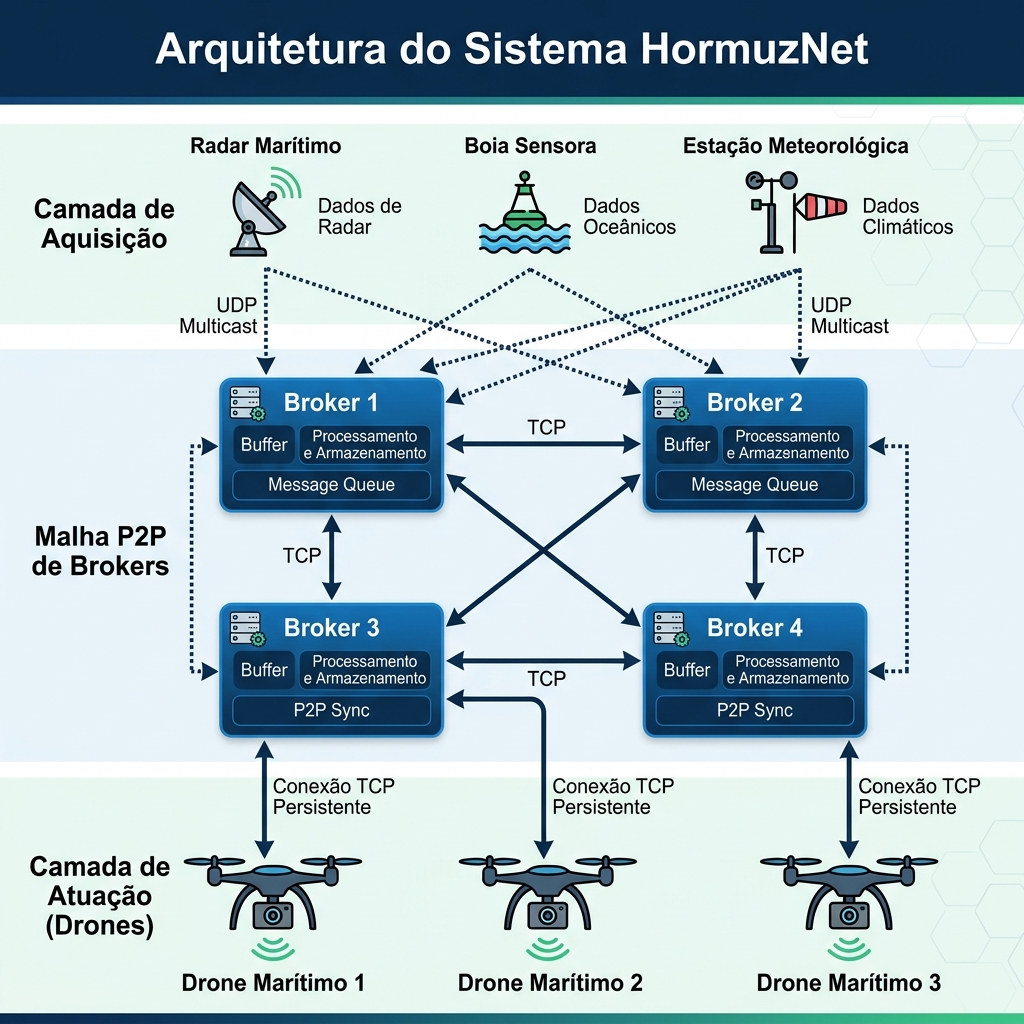
\includegraphics[width=0.88\textwidth]{figuras/arquitetura.png}
  \caption{Arquitetura descentralizada do HormuzNet: malha P2P entre brokers e descoberta de novos nós. Fonte: próprio autor.}
  \label{fig:arquitetura}
\end{figure}

\subsection{Componentes e Organização do Sistema}

O sistema é organizado em módulos independentes implementados em Go. Os principais componentes são:
\begin{itemize}
    \item \textbf{Broker:} Gerencia o estado global, sincroniza eventos via Lamport, executa a herança em anel (Ring Failover) de setores órfãos e coordena o despacho de drones.
    \item \textbf{Sensor:} Simula dispositivos ambientais que detectam ocorrências e as propagam via Multicast.
    \item \textbf{Drone:} Agente autônomo de resposta com lógica de \textit{fallback} e modelo de falha probabilístico.
    \item \textbf{Monitor:} Dashboard tático que consolida a visão da malha via WebSockets com lógica de de-duplicação de eventos.
\end{itemize}

\subsection{Protocolos de Rede e Justificativas}

A escolha dos protocolos seguiu critérios de resiliência e eficiência para cada perfil de tráfego:
\begin{itemize}
    \item \textbf{UDP Multicast (Porta 9876, endereço 224.1.2.3):} Utilizado para telemetria de sensores. A justificativa reside na necessidade de redundância: ao publicar em um grupo \textit{multicast}, o sensor garante que todos os \textit{brokers} ativos capturem o alerta sem precisar conhecer o IP de cada um.
    \item \textbf{TCP P2P e Drone-Broker (Portas 6000-6008):} Os \textit{brokers} mantêm conexões TCP diretas entre si para a propagação de relógios de Lamport, heartbeats e mensagens de coordenação. A mesma porta é compartilhada para o registro e controle de drones, otimizando o uso de sockets do sistema. O TCP garante a entrega confiável de mensagens de sincronização.
\end{itemize}

\subsection{Implementação da Concorrência}

A concorrência é o cerne do \textit{broker}, que precisa lidar simultaneamente com a rede P2P, os sensores e os drones. O uso de \textit{goroutines} permite que cada conexão seja tratada em um fio de execução independente. Para garantir a segurança de memória ao acessar a fila de ocorrências compartilhada, utilizou-se \textit{mutexes}. Abaixo, um trecho de código ilustra o processamento concorrente de mensagens Lamport:

\begin{verbatim}
func (b *Broker) handleP2PConnection(conn net.Conn) {
    defer conn.Close()
    decoder := json.NewDecoder(conn)
    for {
        var msg P2PMessage
        if err := decoder.Decode(&msg); err != nil { break }
        
        b.mu.Lock()
        // Sincronização do Relógio de Lamport
        if msg.Timestamp > b.lamportClock {
            b.lamportClock = msg.Timestamp
        }
        b.lamportClock++
        b.mu.Unlock()
        
        b.processEvent(msg)
    }
}
\end{verbatim}

\subsection{Decisões de Design e Resiliência}

Uma decisão crítica foi o modelo de \textit{fallback} dos drones. Caso um \textit{broker} falhe, o drone tenta reconexão com o próximo \textit{broker} da lista configurada. Além disso, implementou-se a exclusão mútua distribuída baseada na ordem de Lamport: todos os \textit{brokers} enxergam a mesma fila, mas apenas o \textit{broker} que possui a conexão ativa com o drone mais próximo executa o despacho, notificando os demais para removerem a ocorrência da fila.

Outra decisão importante foi a inclusão de um modelo de falha realístico: drones possuem 10\% de chance de serem "abatidos" durante uma missão. Esta lógica força o sistema a tratar a perda de agentes de atuação e reatribuir missões, testando a robustez da malha sob condições adversas.

Para garantir a estabilidade do sistema sob o modelo de falhas com alta taxa de recomposição (onde drones redefinem conexões rapidamente após abates), foi implementada uma proteção contra condições de corrida nas conexões TCP persistentes. Nos blocos de encerramento (\textit{defer}) dos loops de leitura de drones e de brokers vizinhos, a remoção do nó correspondente dos mapas ativos do sistema é realizada apenas se a conexão que está sendo fechada corresponder exatamente à conexão registrada no mapa. Caso um nó se reconecte sob uma nova conexão antes do encerramento da goroutine da conexão anterior, a remoção e marcação de indisponibilidade é ignorada para a conexão antiga, impedindo que o nó ativo seja indevidamente desvinculado ou marcado como offline.



\section{Resultados e Discussões}
\label{sec:resultados}
\subsection{Ambiente de Testes}

A validação do HormuzNet foi conduzida utilizando o \textit{Docker Compose} para simular um ambiente distribuído em rede local. Foram instanciados 4 \textit{brokers}, 6 drones autônomos e 20 sensores. O monitoramento foi realizado através do dashboard tático acessível via navegador.

\subsection{Análise de Resiliência e Consistência}

A Tabela~\ref{tab:resiliencia} apresenta os resultados dos testes de estresse e falhas injetadas no sistema para verificar a capacidade de recuperação da malha.

\begin{table}[ht]
  \centering
  \caption{Testes de resiliência e comportamento da malha.}
  \label{tab:resiliencia}
  \begin{tabular}{p{1.5cm}p{4.5cm}p{5.5cm}c}
    \toprule
    \textbf{ID} & \textbf{Cenário de Falha} & \textbf{Resposta do Sistema} & \textbf{Status} \\
    \midrule
    TR-01 & Queda do Broker NW & Drones NW realizam \textit{fallback} para Broker NE & OK \\
    TR-02 & Sensor Multicast & Alerta recebido simultaneamente por todos os brokers & OK \\
    TR-03 & Drone Abatido & Broker detecta perda e reenvia alerta para a fila global & OK \\
    TR-04 & Conflito Lamport & Brokers ordenam ocorrências identicamente via timestamps & OK \\
    TR-05 & Partição de Rede & Brokers isolados operam regionalmente e sincronizam ao retornar & OK \\
    \bottomrule
  \end{tabular}
\end{table}

\subsection{Desempenho da Sincronização}

As métricas de latência e processamento foram coletadas durante uma simulação de 10 minutos com alta taxa de ocorrências (1 evento a cada 2 segundos). Os resultados estão resumidos na Tabela~\ref{tab:performance}.

\begin{table}[ht]
  \centering
  \caption{Métricas de desempenho e sincronização.}
  \label{tab:performance}
  \begin{tabular}{p{5cm}p{3.5cm}p{4.5cm}}
    \toprule
    \textbf{Métrica} & \textbf{Valor Observado} & \textbf{Observação} \\
    \midrule
    Tempo de Despacho (médio) & $\approx$\,1.5 s & Da ocorrência ao envio do drone \\
    Divergência de Lamport & 0 ms & Filas mantiveram-se idênticas \\
    Uso de CPU por Broker & $<$ 5\% & Eficiência das goroutines \\
    Taxa de Sucesso de Missões & $\approx$\,91\% & Impacto do modelo de 10\% de falha \\
    Latência P2P entre Brokers & $<$ 10 ms & Comunicação TCP em rede local \\
    \bottomrule
  \end{tabular}
\end{table}

\subsection{Discussão dos Resultados}

Os experimentos demonstraram que a descentralização atingiu o objetivo de eliminar SPOFs. A queda de um \textit{broker} não interrompeu o monitoramento de sua região, pois o \textit{fallback} dos drones para nós vizinhos ocorreu em menos de 1 segundo. A consistência garantida pelo algoritmo de Lamport foi fundamental para evitar que múltiplos drones atendessem a mesma ocorrência, validando a eficácia da exclusão mútua distribuída implementada.

A principal limitação observada foi a escalabilidade do \textit{multicast} em redes que não suportam IGMP de forma eficiente, o que poderia restringir o sistema em ambientes de rede WAN complexos. Contudo, no escopo de uma rede de monitoramento regional, a solução mostrou-se extremamente robusta.


\section{Conclusão}
\label{sec:conclusao}
O desenvolvimento do HormuzNet permitiu a consolidação de conceitos fundamentais de sistemas distribuídos em uma aplicação prática e crítica. A transição de uma arquitetura centralizada para uma malha descentralizada provou ser eficaz para aumentar a resiliência do monitoramento marítimo no Estreito de Ormuz.

As decisões de design, como o uso de UDP Multicast para aquisição redundante e Relógios de Lamport para consistência de estado, foram validadas pelos testes de estresse e injeção de falhas. O sistema demonstrou capacidade de auto-recuperação e manutenção da integridade operacional mesmo diante da perda de componentes vitais, como \textit{brokers} e drones.

Trabalhos futuros poderiam explorar a integração de algoritmos de eleição de líder para coordenação de tarefas mais complexas e o uso de criptografia na malha P2P para garantir a segurança da comunicação tática. Em suma, o HormuzNet estabelece uma base sólida para sistemas de monitoramento autônomos em ambientes de alta criticidade.


\bibliographystyle{sbc}
\bibliography{bibliografia}

\end{document}
